
%\documentclass[conference]{IEEEtran}
\documentclass{sig-alternate}

\clubpenalty=10000
\widowpenalty = 10000

\newcommand{\todo}[1]{\textcolor{cyan}{\textbf{[#1]}}}
\newcommand{\sam}[1]{\textcolor{red}{{\it [Sam says: #1]}}}
\newcommand{\dan}[1]{\textcolor{blue}{{\it [Dan says: #1]}}}


\usepackage{cite}
\usepackage{listings}
%\usepackage{booktabs}
\usepackage{color}
\usepackage{balance} % Helps to balance out text on last page
\usepackage{url}
\usepackage{times} % Used for formatting formatting url footnotes
\urlstyle{same} % Used for formatting formatting url footnotes

\usepackage{graphicx} % Including images


\usepackage{tikz}
\usetikzlibrary{shapes, 	arrows, positioning}
\usetikzlibrary{patterns}

\pdfpagewidth=8.5in
\pdfpageheight=11in



\lstset{ %
language=,                % Make language be nothing
basicstyle=\footnotesize,       % the size of the fonts that are used for the code
%numbers=left,                   % where to put the line-numbers; possible values are (none, left, right)
%numberstyle=\tiny\color{gray}, % the style that is used for the line-numbers
stepnumber=1,                   % the step between two line-numbers. If it is 1 each line will be numbered
numbersep=-3pt,                  % how far the line-numbers are from the code
backgroundcolor=\color{white},  % choose the background color. You must add \usepackage{color}
showspaces=false,               % show spaces adding particular underscores
showstringspaces=false,         % underline spaces within strings
showtabs=false,                 % show tabs within strings adding particular underscores
frame=single,           % adds a frame around the code
tabsize=2,          % sets default tabsize to 2 spaces
captionpos=b,           % sets the caption-position to bottom
breaklines=true,        % sets automatic line breaking
breakatwhitespace=false,    % sets if automatic breaks should only happen at whitespace
escapeinside={\%*}{*)}          % if you want to add a comment within your code
}

\begin{document}

\title{Concolic Analysis for Android Applications}



\numberofauthors{1} 
\author{
\alignauthor
Daniel~E.~Krutz, Patrick McAfee, \&~Samuel~A.~Malachowsky\\ 	
	\affaddr{Software Engineering Department}\\
       \affaddr{Rochester Institute of Technology}\\
       \affaddr{1 Lomb Memorial Drive}\\
       \affaddr{Rochester, NY, USA} \\
       \email{\{dxkvse, pjm4439, samvse\}@rit.edu}
       \alignauthor
} % Must not be a space above this

\maketitle

\begin{abstract}

Mobile computing has become an important part of our everyday lives, and the Android operating system has grown to be the most popular mobile platform. Unfortunately, Android applications are not immune to bugs, security vulnerabilities, and a wide range of other issues, a common theme in all software. Concolic analysis, a hybrid software verification technique which performs symbolic execution along a concrete execution path, has been used for a variety of purposes including software testing, code clone detection, and security-related activities.

We created a new publicly available concolic analysis tool for analyzing Android applications: Concolic Analysis for Android (CAA). Building on Java Path Finder (JPF), this tool performs concolic analysis on a raw Android application file (or source code) and provides output in a useful and easy to understand format. Included in this paper are an introduction to the root concepts, a description of the tech stack used within the tool, and basic usage instructions. The tool, detailed instructions, and source code is available on the project website:~\url{http://darwin.rit.edu/caa/}. 


\end{abstract}
% ? Add back in for IEE
%%\IEEEpeerreviewmaketitle

\section{Introduction}

% Describe the problem and then really drive home the value of the tool
% State a problem with much of the software?

Android has grown to become an extremely popular mobile platform with a wide variety of applications (apps) varying in genre, function, and quality. As with all software, Android apps routinely suffer from bugs and security vulnerabilities. Static analysis tools can be extremely beneficial in assisting with these issues and can often quickly and accurately identify issues that developers would have otherwise missed~\cite{Ware:2008:SJC:1394504.1394506, Feng:2014:ASD:2635868.2635869}.

Concolic analysis is a power static analysis technique which has been traditionally used for software testing~\cite{Sen:2005:CCU:1081706.1081750}, security related activities~\cite{Chen:2014:CIB:2554850.2554875}, and code clone detection~\cite{Krutz_Sac15, krutz2013code}. While there are a few concolic analysis tools for Java, none are immediately compatible with Android source code. Traditional concolic tools such as JPF~\cite{visser2003model} and CATG\footnote{\url{https://github.com/ksen007/janala2}} will not work on Android applications because the apps lack a main method which is typically required for concolic analysis tools. We are proposing a new tool, Concolic Analysis on Android (CAA), which allows users to perform concolic analysis on Android application (.apk) source files with ease and without the need for a physical Android device or emulator. The tool not only includes the benefits of concolic static analysis, but provides concolic output which may be important for future work in clone detection and other comparison techniques~\cite{Krutz_Sac15, 6671332,Anand:2012:ACT:2393596.2393666}.

The CAA tool executes seven primary steps: (1) Unpacking the Android application, (2) Conversion of APK into a .jar file, (3) Analysis of entry points into the application, (4) Creation of a wrapper for the decompiled APK, (5) Creation of configuration files for concolic analysis tool, (6) Running JPF, and (7) Logging output from JPF.

%%% Removed for space reasons 3/26
In the following work, we describe the need for our tool, provide details about the application and its design, and include basic usage instructions. The source code of CAA, installation instructions and further results may be found on our website\footnote{\url{http://darwin.rit.edu/caa/}}.

% In the following sections, we will provide an overview of CAA's architecture, usage instructions, output and results.



\section{Related Work}
\label{sec: relatedwork}

There are an assortment of concolic tools which have been created for Java and C based applications. Some include JPF, CREST\footnote{\url{https://code.google.com/p/crest/}}, CATG, and CUTE\cite{Sen:2005:CCU:1081706.1081750}. There are also several proposed techniques for applying concolic analysis to Android and mobile applications. Anand et al.\cite{Anand:2012:ACT:2393596.2393666} created a method known as ACTEve with a goal of alleviating the path-explosion problem with concolic analysis. ACTEve is focused on event-driven applications such as smartphone applications and uses concolic analysis in order to generate feasible event-sequences for Android apps. Unfortunately this approach is often limited to short event sequences due to the resources required.  

As with our tool, JPF-Android~\cite{vanderMerwe:2014:EPS:2557833.2560576} verifies Android apps using JPF. A primary benefit of this technique is that it allows Android applications to be verified outside of any emulator using JPF. While this work is profound, it differs from our tool in that it does not use concolic analysis to perform model checking and produces far different output than our tool. Mirzaei et al.\cite{Mirzaei:2012:TAA:2382756.2382798} described a process of testing Android applications through symbolic execution using custom Android libraries for JPF and simulated events through program analysis. While this work is substantial, it does not discuss the use of concolic analysis and does not appear to have been publicly released as a fully functional tool.

While none use concolic analysis, there are other powerful testing tools for Android apps. Dynadroid\footnote{\url{https://code.google.com/p/dynadroid/}} is a tool for creating inputs to unmodified Android apps.  Google's own testing framework is also available to developers\footnote{\url{http://developer.android.com/tools/testing/testing_android.html}}.



\section{Concolic Analysis}
\label{sec: concolicanalysis}

%%% Removed for space reasons 3/26
%Symbolic analysis is used to execute a program using symbolic inputs utilizing~\emph{path conditions} which are updated whenever a branch of the source code is executed. Symbolic values are used in place of actual, concrete values to represent the variables of the target application~\cite{King:1976:SEP:360248.360252,Cadar:2011:SES:1985793.1985995}. Symbolic analysis has been traditionally used for testing applications finding defects and assisting with the creation of unit tests. A primary drawback of symbolic analysis is the~\emph{path explosion} problem which is the creation of a large, or impractical number of paths for symbolic analysis to follow. \dan{leave this section in about symbolic analysis. I could probably shorten it to a single sentence}


Concolic analysis uses the combination of concrete and symbolic values to analyze software and has been used for testing: assisting with unit test creation, identification of software clones, and the discovery of security vulnerabilities~\cite{Sen:2005:CCU:1081706.1081750, Godefroid_automatedwhitebox, 6671332, Krutz_Sac15}. Concolic analysis was introduced by Sen et al.~\cite{Sen:2005:CCU:1081706.1081750} in 2005, and has an advantage over symbolic analysis since the combination of concrete and symbolic values can be used to simplify constraints and precisely reason about complex data structures~\cite{4222603}.

When an application is executed using concolic analysis, the execution path along with symbolic constraints are stored in the~\emph{path condition}. An execution branch is then selected from this path condition which is provided to the constraint solver to be verified for legitimacy. If correct, concrete test inputs are then used to create a new achievable application path. However, if the new path is found to be unachievable, another application path is then selected. Using this process, concolic analysis attempts to traverse as many paths of the application as possible while limiting the path explosion problem through its use of concrete values~\cite{Jaffar:2013:BCT:2491411.2491425}.


%%% This section was taken from an aborted ICSE NIER paper
%Concolic analysis combines concrete and symbolic values in order to traverse all possible paths of an application (up to a given length). Concolic analysis is a variation of symbolic analysis were concrete executions are simultaneously run with symbolic analysis. In order to examine application paths, solvers are generated which are used to generate new test input to direct the application along the various execution paths. This process is continued until all possible distinct paths have been reached using a depth search strategy~\cite{Sen:2005:CCU:1081706.1081750}. The use of concrete values represents the primary advantage of using concolic analysis instead of symbolic analysis since constraints may be simplified which may assist in the precise reasoning of complex data structures. Concolic analysis has been traditionally used for testing due to its ability to traverse a large number of application paths~\cite{Majumdar:2007:HCT:1248820.1248874}. 


%%% This was all taken from diss



As an example, Listing~\ref{lst:RawCodeToHaveCAAOnIt} displays a function which is to have concolic analysis performed upon it, and Figure~\ref{fig:CAAAnalysisFlow} shows its data flow. The analysis process would first begin with an arbitrary value being assigned to \texttt{a} and \texttt{b}. For the concrete execution, \texttt{a}=\texttt{b}=1. Line \#2 would set \texttt{c} to be 2, and the~\emph{if} statement in the 3rd line will fail since $ \texttt{a} \neq 100000$. The symbolic execution will follow the same path taken by the concrete execution, but will merely treat \texttt{a} and \texttt{b} as symbolic variables. \texttt{C} will be set to the expression 2b and will make note that $ \texttt{a} \neq 100000$ since the test in line 3 failed. This is known as a path condition and will need to be true for every execution following this same path. The goal is to examine every path of the application.

% Not sure if examine should be the correct word

%This means that the next step for this example is to take the last path condition encountered, a ≠ 100000 and negate it. This means that a=100000. In order to find values for the input variables a and b, an automated theorem prover is then invoked using a complete set of symbolic and path variables created during the symbolic execution process. This automated theorem prover shows the logical consequence of a set of statements. The goal of this prover is to help ensure that all program paths are properly followed. In this situation, the values created by this theorem prover may be a=100000 and y =0. Using this input, the application may now reach the inner branch on line 4. Since 100000 is not less than 2, this branch will not be taken. This means that the path conditions are now a=100000 and a ≥ c, which will be negated to have the other path followed meaning that a<c. The theorem prover will next examine a and b to satisfy a=100000, a<c and x=2b. One example of this may be a=100000 and b=50001. Using these assumptions, the error on line 5 will be reached and all possible paths will have been followed.


%\begin{figure}[ht!]
%\centering
%%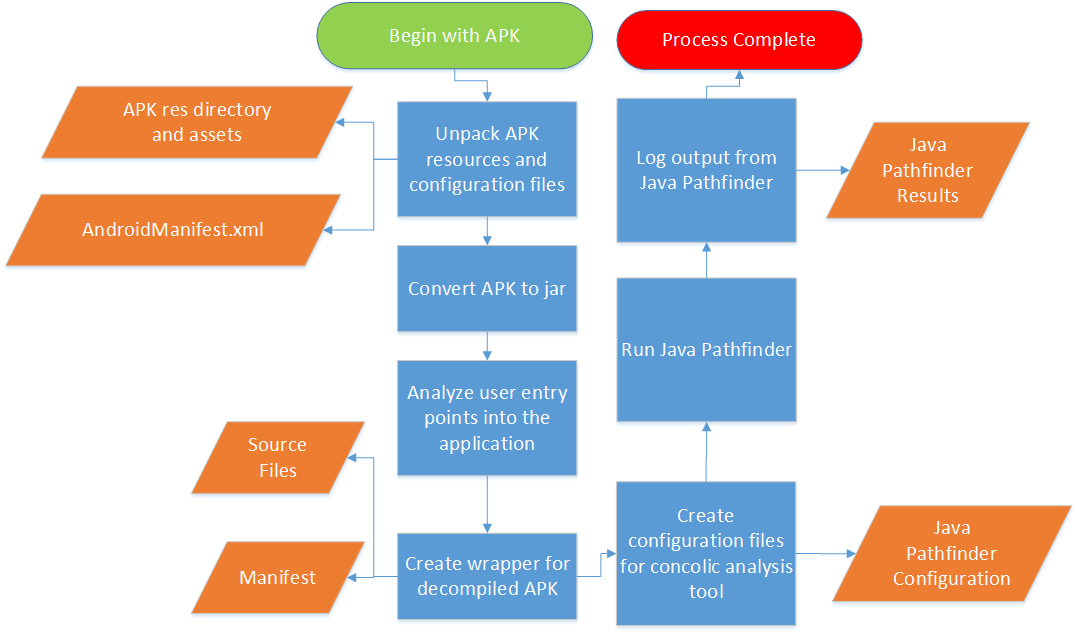
\includegraphics[width=1.0\textwidth]{images/workflow.png}
%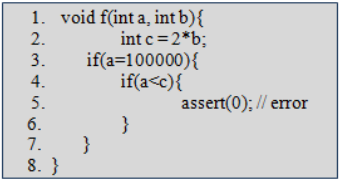
\includegraphics[width=7cm,height=8cm,keepaspectratio]{images/CodeToHaveCAOnIt.png}
%\caption{Concolic Analysis Flow \todo{make this latex}}
%\label{fig:RawCodeToHaveCAAOnIt}
%\end{figure}


\begin{lstlisting}[label=lst:RawCodeToHaveCAAOnIt, caption=Code to be examined by Concolic Analysis, language=Java, numbers=left]
	void f(int a, int b){
		int c = 2*b;
		if(a=100000){
			if(a<c){
				assert(0); //error
			}
		}
	}
\end{lstlisting}




\begin{figure}[h] %h for here, t for top, b for bottom

\begin{center}
% Define block styles
\tikzstyle{round} = [circle, draw, fill=white!20, node distance=1.0cm, text width=3em, text badly centered, align=center]
\tikzstyle{biground} = [circle, draw, fill=white!20, node distance=1.0cm, text width=4em, text badly centered, align=center]
\tikzstyle{line} = [draw, -latex']

\begin{tikzpicture}[node distance = 2.0cm, auto]

\node [round] (1st) {if};
\node [round, below left=1cm of 1st] (2nd) {a=0 b=0};
\node [round, below right=1cm of 1st] (3rd) {if};
\node [biground, below left=1cm of 3rd] (4th) {a=100000 b=0};
\node [biground, below right=1cm of 3rd] (5th) {a=100000 b=50001};

\path [line] (1st) -- node[above left] {$ a \neq 100000$} (2nd);
\path [line] (1st) -- node[above right] {a = 100000} (3rd);
\path [line] (3rd) -- node[above left] {$a \geq c$ } (4th);
\path [line] (3rd) -- node[above right] {a < c} (5th);

\end{tikzpicture}
\caption{Concolic Analysis Flow}
\label{fig:CAAAnalysisFlow}
\end{center}
\end{figure}

Concolic analysis serves as the foundation of the CAA tool, which is described in the next section. 

%\sam{I added this simple transition.  What do you think?}\dan{What if we just said..``Concolic analysis is the important basis of the CAA tool''}

\section{Concolic Analysis for Android (CAA) Tool}
\label{sec: caa}

The core of CAA is based on linking several previously existing tools together in order to provide a framework where concolic analysis can be run with a single process. CAA is designed as an automated toolchain, utilizing other disparate tools to do the more complex tasks. They are as follows:

\begin{itemize}
    \setlength{\itemsep}{0pt} %Cut down on spacing for the different items in the list
    \setlength{\parskip}{0pt} %Cut down on spacing for the different items in the list
    \setlength{\parsep}{0pt}  %Cut down on spacing for the different items in the list
    
%1
\item~\textbf{Apktool}\footnote{\url{https://code.google.com/p/android-apktool/}}: A utility for decompiling APK files into standard Java .jar files.

%2
\item~\textbf{Dex2Jar}\footnote{\url{https://code.google.com/p/dex2jar/}}: A Java utility for decompiling Android applications. This tool extracts the UI resources and other assets from the .jar file, as well as decrypting the AndroidManifest.xml file.

%3
\item~\textbf{Robolectric}\footnote{\url{http://robolectric.org/}}: A library specially designed to stub and mock out the Android runtime when testing a project outside of a standard runtime environment. In the context of this project, it is used to grant access to code paths during concrete execution that other would be unreachable without that framework.

%4 - JPF
\item~\textbf{JPF}\cite{visser2003model}: Performs the actual concolic analysis.  While there are other tools that provide this functionality against vanilla .jar files, such as jCUTE\footnote{\url{http://osl.cs.illinois.edu/software/jcute/}} and CATG, JPF is a best fit for this project, particularly due to its Symbolic optional module which includes the actual concolic analysis. Additionally, it is actively supported with a robust development community (including NASA), which was critical to this project's development. One feature that other tools did not include was the ability to configure a flexible classpath at runtime with multiple directories. This functionality was required for the dynamic compilation described in the design portion of this work.
\end{itemize}

%%% Removed for space reasons 3/26
There were several hurdles we had to overcome in the creation of our tool. First, the Android SDK does not support calls to arbitrary main functions, so it is therefore necessary to provide a wrapper for a decompiled Android APK file. This provides a single input to be used as the the root node for the concolic parser's tree. Second, Android applications are not designed to be run outside an Android runtime, and the provided Android development libraries are insufficient as they are only stubs. This obstacle was overcome through the use of Robolectric, a dynamic Android mocking library which allows for greater coverage of Android code paths.

\subsection{Overview of Architecture}



CAA accepts a path to an APK and executes a linear series of steps to provide the results of concolic analysis.  A high level overview of the process is described below and is shown in Figure~\ref{fig:workflow}.

\begin{figure}[h] %h for here, t for top, b for bottom

\begin{center}
% Define block styles
\tikzstyle{block} = [rectangle, draw, fill=white!20, node distance=1.0cm, text width=11em, text centered, rounded corners, align=center]
\tikzstyle{line} = [draw, -latex']

\begin{tikzpicture}[node distance = 2.0cm, auto]

\node [block] (init) {Begin with APK};
\node [block, below of=init] (1st) {Unpack APK resources and configuration files};
\node [block, below of=1st] (2nd) {Convert APK to .java \& .class};
\node [block, below of=2nd] (3rd) {Analyze user entry points into the application};
\node [block, below = 0.3cm of 3rd] (4th) {Create wrapper for decompiled APK};
\node [block, below = 0.3cm of 4th] (5th) {Create configuration files for concolic analysis tool};
\node [block, below of=5th] (6th) {Run Java Pathfinder};
\node [block, below of=6th] (7th) {Log output from Java Pathfinder};
\node [block, below of=7th] (8th) {Process Complete};

\node [block, dashed, right = 0.6cm of 1st] (1a) {APK res directory and assets};
\node [block, dashed, below of=1a] (1b) {AndroidManifest.xml};
\node [block, dashed, right = 0.6cm of 3rd] (4a) {Source Files};
\node [block, dashed, below of=4a] (4b) {Manifest};
\node [block, dashed, right = 0.6cm of 5th] (5a) {Java Pathfinder Configuration};
\node [block, dashed, right = 0.6cm of 7th] (7a) {Java Pathfinder Results};

\path [line] (init) -- (1st);
\path [line] (1st) -- (2nd);
\path [line] (2nd) -- (3rd);
\path [line] (3rd) -- (4th);
\path [line] (4th) -- (5th);
\path [line] (5th) -- (6th);
\path [line] (6th) -- (7th);
\path [line] (7th) -- (8th);

\path [line, dashed] (1st) -- (1a);
\path [line, dashed] (1st) -- (1b);
\path [line, dashed] (4th) -- (4a);
\path [line, dashed] (4th) -- (4b);
\path [line, dashed] (5th) -- (5a);
\path [line, dashed] (7th) -- (7a);

\end{tikzpicture}
\caption{CAA Workflow}
%\label{fig:CAAWorkflow}
\label{fig:workflow}
\end{center}
\end{figure}





\begin{enumerate}
    %\itemsep-.2em %  \itemsep0em  %% This was the setting that was originally used

    \setlength{\itemsep}{0pt} %Cut down on spacing for the different items in the list
    \setlength{\parskip}{0pt} %Cut down on spacing for the different items in the list
    \setlength{\parsep}{0pt}  %Cut down on spacing for the different items in the list

 \item Unpack APK resources and configuration files
 \item Convert APK .dex files to Java .class files
  \item Analyze user entry points into the application
 \item Create wrapper for decompiled APK
 \begin{enumerate}
\itemsep-.2em %  \itemsep0em
 	\item Create java source files for wrapper from templates
 	\item Fill templates with entry point information and calls
 	\item Compile the wrapper
 \end{enumerate}
 \item Create configuration files for concolic analysis tool
 \item Run JPF
 \item Log output from JPF
 \end{enumerate}



The first step of the process uses Apktool to produce the assets and configuration files which are crucial for Robolectric to run correctly later in the process. All the extracted files are placed in a special directory for later manipulation along with a copy of the targeted APK file.  All subsequent modification is done in this directory.

The second step utilizes Dex2Jar to produce the necessary Java .jar files from the APK file. The .jar format is required for later compilation and manipulation by the CAA tool. It exposes access to the internal code in a way that standard Java tools can easily work with.  It can also provides readable source code, an invaluable resource during development. This jar is also stored within the spawn directory.

The third step is analyzing the provided source from the generated jar file. Through the use of reflection, each class is dynamically loaded and analyzed for known inputs, such as an OnCreate method of an activity. A blocklist is used to prevent excessive automated analysis of the Android libraries themselves, which are dynamically loaded to a custom classpath so that proper matching can happen.  The types of inputs found are used to determine what functions need to be called and what kind of data they need to be sent by CAA and JPF. 


The fourth and most complex step creates a custom wrapper jar against the created jar. Several template files are used to create raw Java source files with tokens.  These tokens are replaced by a source writer in CAA, which interprets the analysis from the previous step.  Calls to supported functions that the framework or user would trigger manually are automated in the source files.  There are two .java files and and a manifest file created from this process, as well as a .jpf file. The first Java file is a wrapper that makes all of the aforementioned calls to the jar converted from the APK file and wraps those calls in a single function as a JUnit test. Robolectric, the Android mocking library being used, operates as a JUnit TestRunner and thus the wrapper function must be a test to utilize the mocks. The second Java file is the wrapper runner whose purpose is loading the wrapper's tests into JUnit and firing them from inside a single entry point. This entry point is then exposed to JPF and indirectly provides access to the underlying functions from the APK file.  The final file is a custom manifest that references all dependencies as well as the jar converted from the APK.  The newly created Java source and manifest are packaged into a custom wrapper jar to be used in the next step of the process.

The fifth and sixth steps build on part of the fourth. During the creation of files from templates, a .jpf file is created. This .jpf file is used by JPF to store arguments to pass to the concolic tool. In particular, this stores the targeted entry function provided by the wrapper jar, the functions that should have the analysis run on them, and the settings to enable concolic analysis. Finally, the output generated by the tool is saved for the user. A small example of this output is shown in Listing~\ref{lst:concolicoutput}, and more complete results may be found on the project website. This output may be useful to researchers and developers in a variety of ways including clone detection, uncovering defects and analyzing the app's functional flow. 

% How else might this output be useful?
%.... Other static analysis techniques? 


\begin{lstlisting}[label=lst:concolicoutput, caption=Example Concolic Output]
8   checkcast
11  putfield java.util.HashMap.table
14  aload_0
15  iconst_0
16  putfield java.util.HashMap.hashSeed
19  aload_0
20  aconst_null
21  putfield java.util.HashMap.entrySet
24  iload_1
\end{lstlisting}

\subsection{Usage Instructions}

Once downloaded and installed using the instructions provided on our project website (\textbf{\url{http://darwin.rit.edu/caa/}}), the tool may be used with the following command:~\emph{``java -jar CAA-1.0.0.jar \-apk \$PATH\_TO\_APK''} where~\emph{\$PATH\_TO\_APK} is the path to the APK file to be analyzed. A directory named ``spawn'' will be created where several temporary artifacts of the process will be created. Results will be logged in a created directory named ``results'' as text files similar in format to ``\emph{\{\$APK\~FILENAME}\}.jpfout.txt.'' The results directory is located in the same directory as the application. A thorough example set of instructions on running the tool may be found on the project website; an example screenshot is shown as Figure~\ref{fig:usingCAA}.

%% I think this could use more details, but I think the website does a really good job explaining what we are trying to do
%% Make sure the installation instructions are VERY apparent on the website since we are relying upon it.

%%



\begin{figure}[ht!]
\centering
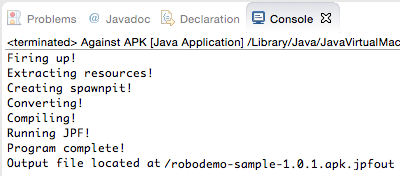
\includegraphics[width=0.45\textwidth]{images/CAA_Eclipse_small.png}
\caption{Example CAA Usage}
\label{fig:usingCAA}
\end{figure}

While there are numerous possible applications of our tool, some immediate uses include gaining a better understanding the functional nature of the app, seeking out redundant functionality, and finding defects.


%%%% If space is an issue, these two sections can be shortened and combined
%\section{Limitations \& Future Work}
%\label{sec: limitations}


\section{Limitations}
\label{sec: limitations}

While CAA represents a powerful and innovative static analysis tool, there are some notable limitations. The targeted coverage is limited to the activity lifecycle startup and is also restricted by the intentional black box testing nature of usage with mocks. The primary issue with the black box nature of this application is that certain Android apps require highly specific data at certain intervals, such as when communicating with servers. Robolectric has no way of knowing what an app expects back from specific calls, and thus cannot correctly mock it out; it can only mock out more simple or common Android API calls. This may cause certain code paths to be excluded from coverage if specific results for calls are expected.

During the creation of tool, the~\emph{Dalvik} runtime was the the only Android runtime. Near the end of development, Android 5.0 was released using the~\emph{ART} runtime. Available APKs are currently theoretically compatible with both and are convertible by Dex2Jar. In the future, this may not be the case as incompatibilities are discovered and the Dalvik runtime becomes antiquated or is no longer supported. Finally, CAA is limited by the tools it relies on and the idiosyncrasies and issues associated with them. As an example, the development of CAA revealed several issues and bugs in JPF's implementation of reflection, some of which are still outstanding and have the potential to affect the reliability of CAA.


\section{Future Work}
\label{sec: futurework}

%%% Removed for space reasons 3/26
There are many improvements that can be made to CAA. As an example, CAA is limited to inefficiently processing one APK file at a time; the concurrent processing of multiple applications would make the usage of the tool more efficient, allowing the application to be more easily utilized by other tools. This change could, for example, allow a user to compare two similar apps and run heuristics on the generated output more quickly (a use case that led to the creation of CAA).

The source writer could also be expanded to provide more coverage. For example, a filter for Android services could be added and the wrapper files could be compiled to target the launch and processing of these application parts. This could then be expanded upon as the Android SDK grows and changes, allowing new entry points and data sources to be covered.

No significant amount of work has been done to compare CAA to other existing Android testing tools. Areas of comparison could include analysis time, amount of code coverage, and precision \& recall of known errors.

\section{Conclusion}
\label{sec: conclusion}
% If needed, this section can be shortened up a bit.

We have presented CAA, a tool that analyzes Android applications using concolic analysis. While there are numerous other testing tools for Android applications (and even some which use concolic analysis), this is the first known freely available tool of its kind which is able to perform concolic analysis using only the source code of the Android application.

%%%%%% Removed for space reasons 3/26
Through a series of seven steps, CAA extracts the source code of the application (using existing tools), dynamically loads the extracted Java class files looking for known inputs which are used in the customer wrapper, then generates the concolic analysis output, which may be used in a variety ways.

We have made the tool, source code, and usage instructions available on our project website:~\textbf{\url{http://darwin.rit.edu/caa/}}. We encourage others to use the tool not only for testing Android applications, but in their research as well.


\balance
\bibliographystyle{abbrv}
\bibliography{CA_Android_tool}

% That's all folks!
\end{document}



% Todo


